% !TEX root =  ../Dissertation.tex

\chapter{Background and Related Work}
\label{ch:background}

This chapter reviews the three key literature I draw on: reservoir computing, regime models in finance, and mixtures of experts together with decision-focused learning. It also presents, in full, the reservoir construction the dissertation uses, since that construction comes directly from the literature rather than from me.

\section{Reservoir computing}
\label{sec:bg-reservoir}

Learning from a time series requires a model that carries information forward in time. Recurrent neural networks do this by passing a state from one step to the next, but training them by propagating gradients back through time is expensive and on short, noisy samples it is also data-hungry. Reservoir computing (RC) is a family of models built around a simple alternative: fix the recurrent part and train only the map that reads it \cite{jaeger2001echo,lukosevicius2009reservoir}. The fixed recurrent network is called the \emph{reservoir}; driven by the input stream it acts as a rich, nonlinear memory, and a simple readout, extracts from its state whatever the task needs.

The best known RC model is the Echo State Network (ESN) \cite{jaeger2001echo}. With input $s(t)$, reservoir state $x(t)$ and readout output $y(t)$, its dynamics and readout are
\begin{equation}
  x(t+1) = f\big(Win s(t+1) + W x(t)+b\big), \qquad y(t+1) = U\, x(t+1),
  \label{eq:esn}
\end{equation}
where $f$ is a sigmoid-type activation, typically $\tanh$. Only $U$ is trained; $W$ and $Win$ are drawn at random and then left alone. For the state to be a usable memory it must be an ``echo'' of the input history rather than of its own arbitrary starting point, the \emph{echo state property}, which is usually arranged by scaling $W$ so that its spectral radius is below one, although that scaling alone is neither necessary nor sufficient \cite{rodan2011simple}. Our system uses a leaky variant of Eq.~\ref{eq:esn}, given later as Eq.~\ref{eq:reservoir}, in which the new state is blended with the old one to lengthen memory.

The standard ESN recipe attracts a standing criticism, set out in \cite{rodan2011simple}: the reservoir is a randomised black box, its properties are poorly understood, getting a good one takes repeated trials and some luck, and the spectral radius is a weak tool for controlling what the dynamics actually do. Prof. Rodan and Prof. Ti\v{n}o therefore asked how much of the randomness and connectivity is necessary at all, and answered: almost none. They study three deterministic templates, a delay line (DLR), a delay line with feedback (DLRB), and the \emph{Simple Cycle Reservoir} (SCR), in which the units form a single ring, every connection in the ring carries the same weight $r$, and every input connection carries the same absolute weight $v$ (Figure~\ref{fig:scr-topologies}). The whole reservoir is then specified by two numbers. Across a wide range of standard benchmarks, NARMA systems, the Santa Fe laser series, the H\'enon map, a nonlinear communication channel, radar and sunspot series, and a speech task, these minimal reservoirs perform comparably to the fully random ESN; on the NARMA family the SCR is the best or statistically not worse than the best.

\begin{figure}[t]
  \centering
  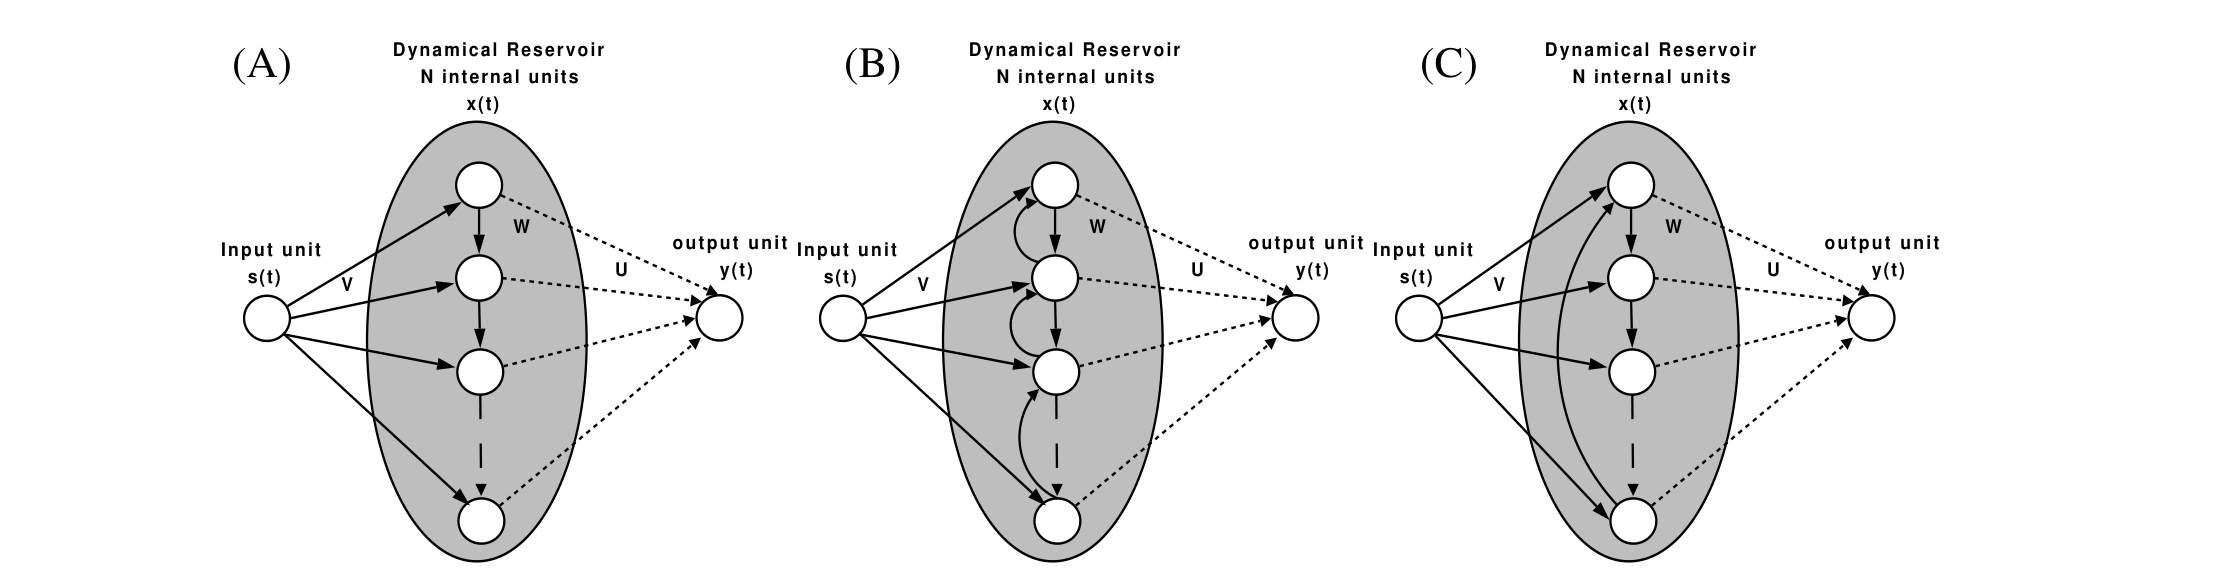
\includegraphics[width=\textwidth]{fig_scr_topologies.png}
  \caption[Minimum-complexity reservoir topologies]{The three
  minimum-complexity reservoir templates :(A) the delay
  line reservoir, (B) the delay line with feedback, and (C) the Simple Cycle
  Reservoir used in this dissertation, in which the units form a single ring
  with one shared weight. Reproduced from Fig.~2 of \cite{rodan2011simple}.}
  \label{fig:scr-topologies}
\end{figure}

One residual source of randomness remains in their construction: the signs of the input weights.Imposing any \emph{periodic} sign pattern hurts performance, but any \emph{aperiodic} pattern works, and it can be generated deterministically, for example by thresholding the decimal digits of $\pi$, digits below five giving a negative sign, or from the digits of $e$, or from a logistic-map trajectory \cite{rodan2011simple}. With that last piece the reservoir contains no randomness at all.

They also characterise what the simplification costs in memory. The short-term memory capacity $MC$ of a reservoir sums, over all delays $k$, the squared correlation between the input delayed by $k$ steps and the network's best reconstruction of it. A classical result of Jaeger bounds $MC \le N$ for any $N$-unit network. For the linear SCR the paper proves the capacity exactly:
\begin{equation}
  MC \;=\; N - \big(1 - r^{2N}\big),
  \label{eq:scr-mc}
\end{equation}
so that choosing $r = (1-\epsilon)^{1/2N}$ places the capacity within any
desired $\epsilon$ of the proven optimum $N$. The ring loses essentially
nothing.

\subsection{Construction of the reservoir matrices}
\label{sec:bg-scr-construction}

This dissertation adopts the SCR construction exactly, writing the cycle
weight as $\rho$ because, for a ring, the shared weight and the spectral
radius coincide. Both matrices are fixed and fully deterministic: nothing here
is trained or drawn at random.

\paragraph{The recurrent matrix $W$ -  a single cycle.}
The $N$ units are wired into one ring with a single shared weight equal to the spectral radius $\rho$. Unit $i$ receives from unit $i-1$, and unit $0$ receives from the last unit, closing the loop:
\begin{equation}
  W_{ij} =
  \begin{cases}
    \rho & \text{if } j \equiv (i-1) \bmod N,\\
    0    & \text{otherwise,}
  \end{cases}
  \qquad
  W = \rho
  \begin{pmatrix}
    0 & 0 & \cdots & 0 & 1\\
    1 & 0 & \cdots & 0 & 0\\
    0 & 1 & \cdots & 0 & 0\\
    \vdots & & \ddots & & \vdots\\
    0 & 0 & \cdots & 1 & 0
  \end{pmatrix}.
  \label{eq:scr-recurrent}
\end{equation}
The nonzeros lie on the sub-diagonal plus the top right corner (the wrap-around). The eigenvalues of such an $N$-cycle are $\rho$ times the $N$-th roots of unity, so every eigenvalue has modulus exactly $|\rho|$ and the spectral radius \emph{is} $\rho$ by construction leading to no rescaling and no eigenvalue solve, we just have this hyperparameter $\rho$.

\paragraph{The input matrix}
Every input connection shares a single magnitude $v$ (the calibrated input
scale); only its sign and the unit it feeds vary.
\begin{equation}
  W_{\mathrm{in}} \;=\; v\,D\,C,
  \label{eq:scr-input-vdc}
\end{equation}
where the sign diagonal $D \in \mathbb{R}^{N\times N}$ and the cyclic
assignment $C \in \{0,1\}^{N\times M}$ are
\begin{equation}
  D =
  \begin{pmatrix}
    s_0 &        &        &        \\
        & s_1    &        &        \\
        &        & \ddots &        \\
        &        &        & s_{N-1}
  \end{pmatrix},
  \qquad
  C =
  \underbrace{
  \begin{pmatrix}
    I_M \\ I_M \\ \vdots \\ I_M
  \end{pmatrix}}_{N/M \text{ copies}},
  \qquad
  s_i =
  \begin{cases}
    +1 & d_i \ge 5,\\
    -1 & d_i < 5,
  \end{cases}
\end{equation}
with $I_M$ the $M\times M$ identity and $d_i$ the $i$-th decimal digit of
$\pi$ \cite{rodan2011simple}, computed from Machin's formula
$\pi = 16\arctan\tfrac{1}{5} - 4\arctan\tfrac{1}{239}$ rather than transcribed.
So unit $i$ listens to input $i \bmod M$ with a fixed $\pm$ sign, and each asset
drives an equal share of the reservoir.

\subsection{Universality of the cycle}
\label{sec:bg-universality}

A fair worry about an architecture so constrained is expressive power: does the ring give something up that a fully random reservoir keeps? For the reservoir class as a whole the answer was already known to be reassuring \cite{grigoryeva2018universal}: reservoir systems are universal approximators of time-invariant fading-memory filters, and universality holds even with \emph{linear} state dynamics provided the trainable readout is rich enough. What remained open was whether the restricted cycle(SCR) retains this power. Li, Fong and Ti\v{n}o \cite{li2024universal} settle it: simple cycle reservoirs, with the ring weight taken complex and input couplings restricted to $\{\pm 1, \pm i\}$, can approximate any unrestricted linear reservoir system with continuous readout to arbitrary accuracy, and therefore any time-invariant fading-memory filter over uniformly bounded inputs.

Two remarks connect these results to the design of this study. First, they are what licenses freezing the encoder: the SCR is not an ad hoc simplification but a construction whose memory is characterised exactly and whose expressive ceiling is known, so the interesting questions move to where the training data are scarcest, the readout and the objective. Second, universality is a statement about sufficiently rich readouts on the frozen state. This dissertation deliberately keeps its readouts \emph{linear}, trading the expressive ceiling for trainability on a few hundred decisions per fold, and that trade has exact consequences: Chapter~\ref{ch:discussion} shows that one family of market features, the even functions of returns that volatility belongs to, is provably out of a linear readout's reach on this state. The same structure that makes the reservoir analysable makes its limits analysable too.

\section{Regime models in finance}
\label{sec:bg-regimes}

The idea that markets move between a small number of conditions is old and well developed. One of this popular statistical form is the Markov switching model of Hamilton \cite{hamilton1989new}, in which an unobserved discrete state follows a Markov chain and the observed series changes its dynamics with the state. Applied to US output, the two recovered states aligned with expansions and recessions. The machinery for such models, filtering, smoothing and EM fitting, is that of hidden Markov models \cite{rabiner1989tutorial}. One key distinction is that the \emph{filtered} state probability uses only observations up to the current day, while the \emph{smoothed} probability conditions on the whole sample, future included. Only the filtered quantity is legitimate in a backtest, and Section~\ref{sec:baselines} implements the HMM gate with a causal filter for exactly this reason.

Ang and Bekaert \cite{ang2002international} document a high-volatility, high-correlation regime in international equity returns, the conditions in which diversification helps least arriving together, and study its consequences for allocation. Guidolin and Timmermann \cite{guidolin2007asset} estimate multivariate regime-switching models for stock and bond returns and find the optimal allocation changes substantially with the regime. Alongside these estimated models sits a simpler tradition that needs no fitting at all: classifying the day by the level of the VIX index. The VIX-tercile gate of Section~\ref{sec:baselines} encodes that heuristic in causal form.

What every scheme in this section shares is the order of operations: the regimes are defined first, from the statistics of returns or from a chosen index, and decisions follow. Whether that order is the right one is precisely what this dissertation asks.

\section{Mixture-of-experts and decision-focused learning}
\label{sec:bg-moe}

The mixture of experts of Jacobs, Jordan, Nowlan and Hinton \cite{jacobs1991adaptive} is the architecture this dissertation uses to make regimes learnable. Several small networks i.e the experts, propose outputs, and a gating network assigns each input a soft weighting over them. Trained together, the gate learns to split the input space and each expert learns to specialise on its share. The regime interpretation is immediate: the gate's weighting \emph{is} a soft regime label, and the experts are per-regime policies. Chapter~\ref{ch:methodology} uses exactly this, with the reservoir state as the gate's input and portfolios as the experts' outputs.

The second ingredient is the objective. The classical portfolio pipeline predicts first and optimises second: estimate expected returns and covariances, then hand the estimates to a mean-variance optimiser. Its known weakness is estimation error, which the optimiser amplifies. The shrinkage covariance estimator of Ledoit and Wolf \cite{ledoit2004honey} is the standard remedy and serves as this study's strongest classical baseline. But a deeper problem remains even with good estimates which is that the forecaster is trained on prediction error, which is only a proxy for decision quality, and the two can disagree, as the worked example of Section~\ref{sec:principle} shows. The decision-focused learning literature addresses this by training the predictor under the loss induced by the downstream decision, the ``Smart Predict-then-Optimize'' framework of Elmachtoub and Grigas \cite{elmachtoub2022smart}. This dissertation takes the idea one step further: it removes the prediction target altogether and trains the portfolio map end to end on the realised risk-adjusted return itself, the excess Sharpe ratio \cite{sharpe1994sharpe}, made differentiable by writing the accounting ledger in the same tensor framework as the model.
